\section{Цифрові датчики}

З попередньої частини про аналогові датчики можна було з'ясувати, що працювати з ними важко, потрібно використовувати складні формули для перетворення напруги в одиниці вимірювання температури, часто потрібно використовувати фільтри сигналу, щоб запобігти значного спотворення сигналу доки він дійде до АЦП. У випадку с термопарою ситуація виходить ще складніша, адже окрім фільтрації потрібно ще знати температуру холодного сплаву, і додавати її або програмним способом, або просто у схемі з'єднавши послідовно термопару та схему компенсації, яка повинна генерувати напругу з тим же шагом (0.4мВ/$^\circ$C) (рис.~\ref{fig:thermocuple_cold_junction_compensation}).
\enlargethispage{\baselineskip}

\begin{figure}[ht]
    \centering
    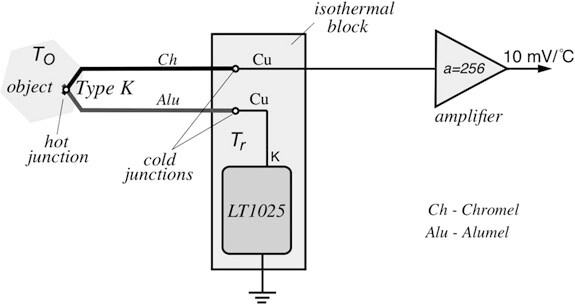
\includegraphics[width=0.8\linewidth]{thermocouple_cj_compensation.jpg}
    \caption{Додавання сигналів з термопари та компенсатора холодного сплаву}
    \label{fig:thermocuple_cold_junction_compensation}
\end{figure}

Ці недоліки, коли потрібна максимальна простота з боку схемотехнічної реалізації та надійність, яку дає виробник, приводить нас до цифрових датчиків. Вони містять у собі АЦП, інтегральну мікросхему, фільтри, і на виході генерують дискретний сигнал, який передають по спеціальних шинах даних стійких до завад (принаймні, на малій відстані). Існує безліч цифрових датчиків, про деякі з них піде річ далі.\\

\textbf{DS18B20}\bigskip

Один з найпопулярніших цифрових датчиків температури, який виробляється фірмою Maxim Integrated. Передача даних відбувається за допомогою пропрієтарної дуплексної шини даних 1-Wire, яка використовує одну лінію для взаємодії з підключеними девайсами. На шину можна під'єднати безліч датчиків, адже кожен з них має свій унікальний номер. Датчик потребує живлення 5В, яке також може подаватися через шину дану (паразитне живлення). Шину даних потрібно підтягнути до живлення резистором ~5 кОм. На рис.\ref{fig:ds18b20_scheme} зображена внутрішня реалізація датчику.

\begin{figure}[ht]
    \centering
    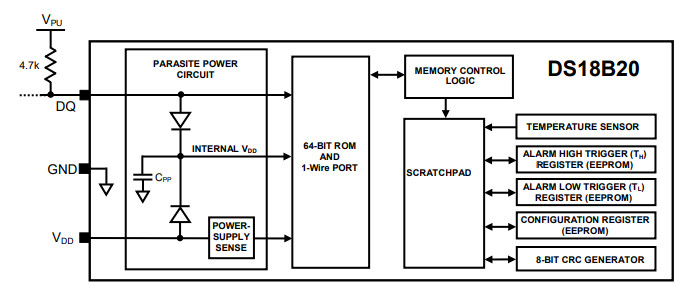
\includegraphics[width=\linewidth]{ds18b20_scheme.jpg}
    \caption{Внутрішня структура DS18B20}
    \label{fig:ds18b20_scheme}
\end{figure}

Датчик здатен вимірювати температуру у діапазоні від -55$^\circ$C до 125$^\circ$C з точністю 0.5$^\circ$C. Роздільну здатність можна також налаштувати від 9 до 12 бітів (за замовчуванням 12), тобто, наприклад 11 бітів відповідають {$\frac{125-(-55)}{2^{11}}~\approx~0.09^\circ$C} ``чутливості''. За специфікацією маємо наступні калібровані значення: 0.5$^\circ$C, 0.25$^\circ$C, 0.125$^\circ$C, 0.0625$^\circ$C. Щобільше обрана розрядність, то повільніше буде вимірювати температуру датчик: 93.75 мс, 187.5 мс, 375 мс, 750 мс.

Після посилання команди на вимір температури, в залежності від розрядності, вимір займе вищевказаний час. Датчик зберігає температуру у 16 бітний регістр, який після вимірювання потрібно зчитувати.

\begin{figure}[ht]
    \centering
    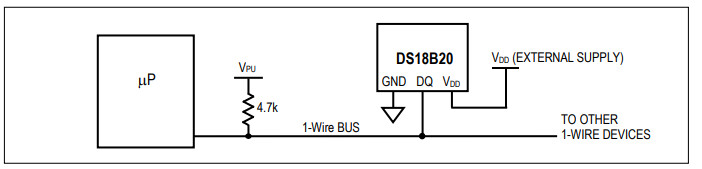
\includegraphics[width=\linewidth]{ds18b20_connect.jpg}
    \caption{Приклад підключення датчика}
    \label{fig:}
\end{figure}

В цілому цей датчик має низьку ціну, дозволяє за допомогою інтерфейсу 1-Wire організувати мережу датчиків, що охоплюють ту чи іншу область. Наприклад, декілька датчиків можна встановити у теплиці та контролювати температуру. Взагалі, саме такі проєкти є головними споживачами цього датчика.\\

\textbf{DHT11}\bigskip

На відміну від попереднього датчика цей є більше простим, але окрім темеператури дозволяє вимірювати вологість. Передача даних відбувається за допомогою однопровідної шини даних використовуючи простий протокол для комунікації. Не підтримує під'єднання декількох датчиків на одну шину.

Може працювати від напруги 3.3 до 5 В. Шина даних підтягується до живлення резистором ~5 кОм. Для вимірювання температури використовує термістор, а коефіцієнти калібрування записані на read-only OTP пам'яті. Точність DHT11 зазвичай становить +/-2$^\circ$C для температури та +/- 5\% для вологості. Роздільна здатність -- 1$^\circ$C. Резистивний елемент, вбудований у датчик, реагує на зміни вологості.

У цьому датчику не має вбудованої пам'яті для збереження результатів вимірювань, а час вимірювання становить 2 секунди, а у найгірших випадках до 30 секунд.

\begin{figure}[ht]
    \centering
    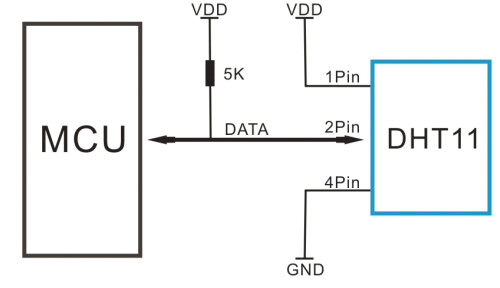
\includegraphics[width=0.6\linewidth]{dht11_connect.jpg}
    \caption{Приклад підключення датчика}
    \label{fig:}
\end{figure}

Взагалі, датчик можна вважати невдалим, і його використання навіть у проєктах теплиці є великим питанням. Має низьку ціну, але водночас усі його характеристики є поганими, порівнюючи з іншими датчиками. Не рекомендується для використання.\\

\textbf{DHT22}\bigskip

Датчик DHT22, також відомий як AM2302, є вдосконаленою версією DHT11, надаючи покращену точність та ряд інших характеристик для вимірювання температури та вологості. Для передачі даних DHT22 використовує простий цифровий інтерфейс, але у порівнянні з DHT11, має меншу частоту оновлення даних, що робить його більш стійким до зовнішніх перешкод.

Побудований також на базі термістора, використовує конденсаторні елементи для вимірювання вологості. Зміна вологості впливає на діелектричні властивості конденсаторів, що визначається мікроконтролером для визначення вологості повітря. На відміну від DHT11 використовує шкалу компенсації температурних змін, що дозволяє коригувати вимірювання вологості в залежності від змін температури, щоб забезпечити точніші результати в різних умовах. Також має певну стійкість до зовнішніх впливів, таких як конденсація водяної пари.

DHT22 вимірює температуру від -40 до 80$^\circ$C та вологість від 0\% до 100\%. Точність DHT22 зазвичай становить +/- 0.5$^\circ$C для температури та +/- 2\% для вологості. Роздільна здатність - 0.1$^\circ$C.

Таким чином, DHT22 є більш розвиненою версією DHT11. Він має вищу точність вимірювань, а також можливості компенсації температурних змін.\\

\textbf{HTU21D}\bigskip

Датчик HTU21D1 є цифровим датчиком вологості та температури, розробленим компанією Measurement Specialties. Він відзначається високою точністю вимірювань та компактним дизайном.

Для передачі сигналу у цифровому сигналі використовує шину I²C, що дозволяє дуже просто його підключати та використовувати багато пристроїв на єдиній шині. Датчик має низьке енергоспоживання (максимальна напруга -- 3.8В, струм у стані спокою -- 0.02 мкА, у стані вимірювання -- до 500 мкА) та є більш чутливим до змін температури. Має високу точність вимірювань. Точність для вологості може сягати до +/- 2\%, а для температури -- до +/- 0.3°C. Не потребує калібрації, адже кожен датчик індивідуально калібрується і тестується. Номер партії друкується на датчику, а його власний ідентифікатор зберігається на мікросхемі, який можна зчитати за допомогою команди. Роздільна здатність може бути змінена за допомогою команди (11 -- 14 бітів для температури та 8 -- 12 для вологості). Тобто роздільна здатність при максимальній розрядності 12 бітів отримаємо роздільну здатність ~ 0.01$^\circ$C.

Датчик забезпечує вимірювання вологості в діапазоні від 0\% до 100\% та температури від -40°C до 125°C. Датчик має вбудований нагрівний елемент, який здатен підвищити температуру на 1.5$^\circ$C. Як і попередній датчик здатен компенсувати температуру при вимірюванні вологості від 0 до 80$^\circ$C.

На відміну від усіх попередніх цифрових датчиків, час виміру температури не перевищує 50 мс при максимальній роздільній здатності.

Специфікація надає формули для виміру приблизної точки роси використовуючи зчитану температуру та вологість (формули \ref{eq:dew_point1}-\ref{eq:dew_point2})

\begin{equation}
    \begin{aligned}
        PP_{Tamb} = 10^{\left[A-\frac{B}{\left(T_{Amb}+C\right)}\right]}
        & \text{ , де T -- виміряна температура} \\
        & \text{A, B, C -- константи 8.1332, 1762.39, 235.66}
    \end{aligned}
    \label{eq:dew_point1}
\end{equation}

\begin{equation}
    \begin{aligned}
        T_d = -\left[\frac{B}{\log_{10} \left(RH_{amb}\cdot\frac{PP_{Tamb}}{100}\right)-A}+C\right]
        & \text{ , де $T_d$ -- точка роси} \\
        & PP_{Tamb} \text{ -- парціальний тиск} \\
        & RH_{amb} \text{ -- вологість повітря}
    \end{aligned}
    \label{eq:dew_point2}
\end{equation}
